\documentclass[aspectratio=43]{beamer}
\usepackage[utf8]{inputenc}
\usepackage[english,russian]{babel}
\usepackage[T2A]{fontenc}


\sloppy

\newcommand{\lama}{$\lambda\kern -.1667em\lower -.5ex\hbox{$a$}\kern -.1000em\lower .2ex\hbox{$\mathcal M$}\kern -.1000em\lower -.5ex\hbox{$a$}$\xspace}

\mode<presentation>{
  \usetheme{IPLC}
}

\begin{document}

\begin{frame}[fragile]{Языки программирования}
  \onslide<2->{
  \begin{columns}
  \column{0.6\textwidth}
  \begin{itemize}      
  \item Синтаксис
    \onslide<3->{\begin{itemize}\item Форма представления программ\end{itemize}}
  \item Семантика
    \onslide<4->{\begin{itemize}\item ``Смысл'' программ\end{itemize}}
  \item Прагматика
    \onslide<5->{\begin{itemize}\item Взаимодействие языка программирования с программистом\end{itemize}}
  \end{itemize}
\column{0.4\textwidth}
\begin{figure}
  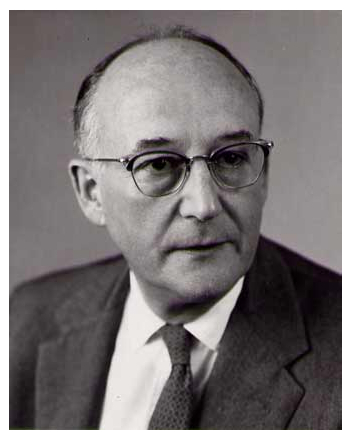
\includegraphics[scale=0.25]{images/morris.jpg}
  \caption{Чарльз Уильям Моррис (1903-1979)}
 \end{figure}
\end{columns}}  
\end{frame}

\begin{frame}[fragile]{Синтаксис}
  \newsavebox{\mybox}
  \begin{lrbox}{\mybox}
    \begin{tikzpicture}
    \node (main) at (0, 0) {
    \begin{lstlisting}[basicstyle=\fontencoding{T1}\footnotesize\fontfamily{lmtt}\fontseries{c}\selectfont,morekeywords={if,else},keywordstyle=\underline]
    if (n > 100) n = 10; else f (f (n + 11));
    \end{lstlisting}};
    \onslide<3->{
    \node at (-3.5, 0.5) {\textit{\textsf{\tiny{ключевое слово}}}};
    \node at (-0.3, 0.4) {\textit{\textsf{\tiny{десятичная константа}}}};
    \node at (-2.8, 0.9) {\textit{\textsf{\tiny{разделитель}}}};
    \node at (-2.5, 1.2) {\textit{\textsf{\tiny{идентификатор}}}};
    \node at (-1.5, 0.7) {\textit{\textsf{\tiny{бинарная операция}}}};
    \draw[-stealth] (-3.4,  0.4) -- (-3.4, 0.2);
    \draw[-stealth] (-2.7,  0.8) -- (-2.7, 0.2);
    \draw[-stealth] (-2.9,  1.1) -- (-2.9, 0.2);
    \draw[-stealth] (-2.3,  0.6) -- (-2.3, 0.2);
    \draw[-stealth] (-1.6, 0.42) -- (-1.8, 0.42) -- (-1.8, 0.2);
    }
    \onslide<4->{
    \node at (0    ,   -1) {\textit{\textsf{\tiny{оператор}}}};
    \node at (-0.35, -0.5) {\textit{\textsf{\tiny{оператор}}}};
    \node at (3    , -0.5) {\textit{\textsf{\tiny{оператор}}}};
    \node at (-2.1 , -0.5) {\textit{\textsf{\tiny{выражение}}}};
    \draw [decorate,decoration = {brace,mirror}] (-3.5, -0.7) -- (4.2, -0.7);    
    \draw [decorate,decoration = {brace,mirror}] (-2.9, -0.2) -- (-1.3, -0.2);    
    \draw [decorate,decoration = {brace,mirror}] (-1, -0.2) -- (0.3, -0.2);    
    \draw [decorate,decoration = {brace,mirror}] (1.6, -0.2) -- (4.2, -0.2);
    }
    \end{tikzpicture}
  \end{lrbox}
  \begin{itemize}
  \item Лексический и грамматический уровень
      \onslide<2->{
      \usebox{\mybox}
      \global\let\mybox\relax}
    \item Однозначность
          \onslide<5->{
    \begin{itemize}\item ``Входя в двери лифта с животными,\\ придерживайте их.''\end{itemize}}
  \item Эффективная распознаваемость
  \end{itemize}  
\end{frame}

\begin{frame}[fragile]{Семантика}
  \newsavebox{\mybox}
  \begin{lrbox}{\mybox}
    \begin{lstlisting}[basicstyle=\fontencoding{T1}\footnotesize\fontfamily{lmtt}\fontseries{c}\selectfont,morekeywords={if,else},keywordstyle=\underline]
      0*(x/0) = ?
      -x+1+x  = ?
      x+1-1   = ?
    \end{lstlisting}
  \end{lrbox}
  \begin{itemize}
  \item Неформальная семантика
    \onslide<2->{
      \begin{itemize}\item ``Выражения состоят из переменных, констант и знаков четырех арифметических действий'' \end{itemize}
      \onslide<3->{\usebox{\mybox}\global\let\mybox\relax}}
      \onslide<4->{\begin{itemize}\item Примеры ``запутанных'' программ: \footnotesize\fontfamily{lmtt}\fontseries{c}\selectfont{https://www.cise.ufl.edu/\textasciitilde manuel/obfuscate/obfuscate.html}\end{itemize}}
  \item Формальная семантика
    \onslide<5->{\begin{itemize}\item Специальная математическая теория\end{itemize}}
  \end{itemize}  
\end{frame}

\begin{frame}[fragile]{Трансляция}
  \begin{itemize}
  \item Трансляция: синтаксическое преобразование программы на одном языке в программу на другом
    \begin{itemize}
      \item Исходный язык: язык, с которого производится трансляция
      \item Целевой язык: язык, в который производится трансляция
      \item Инструментальный язык: язык реализации транслятора
    \end{itemize}
  \end{itemize}  
\end{frame}

\begin{frame}[fragile]{Метапрограммирование}
  kkk
\end{frame}

\end{document}
